\documentclass[12pt]{article}
\usepackage{alltt}
\usepackage[utf8]{inputenc}
\usepackage[dvips]{graphicx}
%\usepackage{a4wide}
\usepackage{epsfig}
\usepackage{fancybox}
\usepackage{verbatim}
\usepackage{array}
\usepackage{latexsym}
\usepackage{alltt}
%\usepackage{dsfont}
\usepackage{caption}
\usepackage{subcaption}
%\usepackage{fullpage}
\usepackage{hyperref}
\usepackage{textcomp}
\usepackage{listings}
\usepackage{color}
\usepackage{amsmath}
\usepackage{amsfonts}
\usepackage{tikz}
\usepackage{float}
\usepackage{matlab-prettifier}
\usepackage{graphicx}

\usepackage[hmargin=3cm,vmargin=6.0cm]{geometry}

\topmargin=-1.8cm
\addtolength{\textheight}{6.5cm}
\addtolength{\textwidth}{2.0cm}
\setlength{\oddsidemargin}{0.0cm}
\setlength{\evensidemargin}{0.0cm}

\newcommand{\HRule}{\rule{\linewidth}{1mm}}

\usepackage{tikz}
\usetikzlibrary{trees}
\tikzset{
  font={\fontsize{7pt}{12}\selectfont}}
  
\newcommand{\Q}{\raisebox{1.7pt}{$\scriptstyle\bigcirc$}}

\lstset{
    %backgroundcolor=\color{lbcolor},
    tabsize=2,
    language=C++,
    basicstyle=\footnotesize,
    numberstyle=\footnotesize,
    aboveskip={0.0\baselineskip},
    belowskip={0.0\baselineskip},
    columns=fixed,
    showstringspaces=false,
    breaklines=true,
    prebreak=\raisebox{0ex}[0ex][0ex]{\ensuremath{\hookleftarrow}},
    %frame=single,
    showtabs=false,
    showspaces=false,
    showstringspaces=false,
    identifierstyle=\ttfamily,
    keywordstyle=\color[rgb]{0,0,1},
    commentstyle=\color[rgb]{0.133,0.545,0.133},
    stringstyle=\color[rgb]{0.627,0.126,0.941},
}

\usepackage[]{mdframed}
\usepackage{enumitem}

\usepackage{titlesec}
\titleformat{\subsection}[runin]{}{}{}{}[]









\begin{document}

% Set the overall layout of the tree
\tikzstyle{level 1}=[level distance=2.5cm, sibling distance=20em]
\tikzstyle{level 2}=[level distance=2.5cm, sibling distance=10em]

% Define styles for bags and leafs
\tikzstyle{bag} = [text width=16em, text centered, align=center]
\tikzstyle{end} = [circle, minimum width=3pt,fill, inner sep=0pt]

\noindent
\HRule \\[3mm]
\small
\begin{tabular}[b]{lp{4.3cm}r}
Middle East Technical University &  &
Department of Computer Engineering \\
\end{tabular} \\
\begin{center}

                 \LARGE \textbf{CENG 280} \\[4mm]
                 \Large Formal Languages and Abstract Machines \\[4mm]
                \normalsize Spring 2022-2023 \\
                    \Large Homework 5 \\
\end{center}
\HRule



% Write down your name, surname, and student ID below.
\begin{center}
Name Surname: Doruk Berke Yurtsizoglu   \\
Student ID: 2522225
\end{center}



\section*{Answer for Q1}

\subsection*{a.} 

Strings that have equal number of 1s and 0s.


\subsection*{b.}    


Yes, it is ambiguous. We can prove this by giving a simple example. If we consider the empty string for this language, it is obvious that it can be produced by both the rule A and B which leads to different parse trees. So, we can say that the language $G_1$ is ambiguous.



\section*{Answer for Q2}

\subsection*{a.} 

We can give an example string and analyze its parse trees, in order to conclude if the given grammar is ambiguous or not.\\
Let's pick the string 'ab', this string has different parse trees:\\
\\
First One:\\

\begin{center}
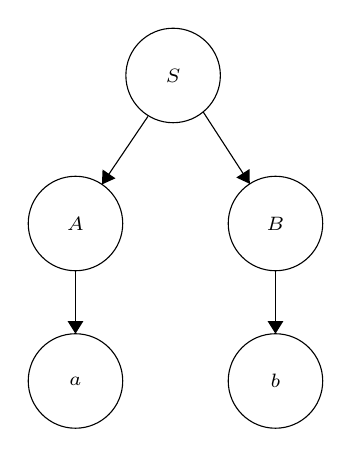
\begin{tikzpicture}[scale=0.2]
\tikzstyle{every node}+=[inner sep=0pt]
\draw [black] (37.9,-8.4) circle (3);
\draw (37.9,-8.4) node {$S$};
\draw [black] (31.7,-17.8) circle (3);
\draw (31.7,-17.8) node {$A$};
\draw [black] (44.4,-17.8) circle (3);
\draw (44.4,-17.8) node {$B$};
\draw [black] (31.7,-27.8) circle (3);
\draw (31.7,-27.8) node {$a$};
\draw [black] (44.4,-27.8) circle (3);
\draw (44.4,-27.8) node {$b$};
\draw [black] (36.3,-11) -- (33.38,-15.32);
\fill [black] (33.38,-15.32) -- (34.24,-14.93) -- (33.42,-14.37);
\draw [black] (39.8,-10.7) -- (42.77,-15.28);
\fill [black] (42.77,-15.28) -- (42.75,-14.34) -- (41.91,-14.88);
\draw [black] (31.7,-20.8) -- (31.7,-24.8);
\fill [black] (31.7,-24.8) -- (32.2,-24) -- (31.2,-24);
\draw [black] (44.4,-20.8) -- (44.4,-24.8);
\fill [black] (44.4,-24.8) -- (44.9,-24) -- (43.9,-24);
\end{tikzpicture}
\end{center}

Second One:\\

\begin{center}
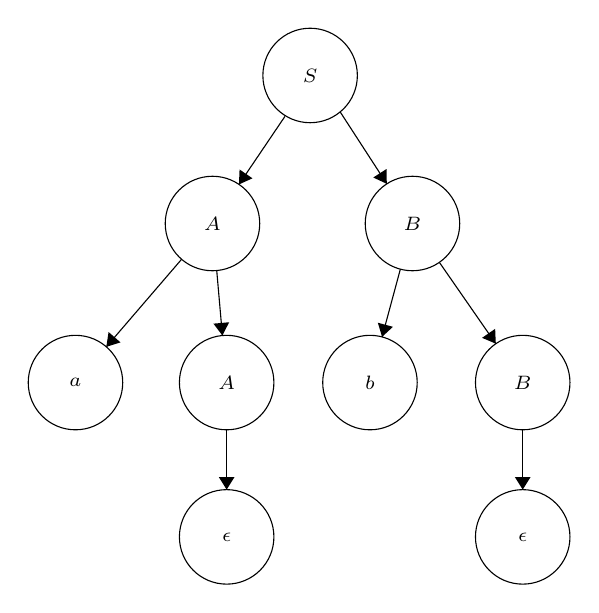
\begin{tikzpicture}[scale=0.2]
\tikzstyle{every node}+=[inner sep=0pt]
\draw [black] (37.9,-8.4) circle (3);
\draw (37.9,-8.4) node {$S$};
\draw [black] (31.7,-17.8) circle (3);
\draw (31.7,-17.8) node {$A$};
\draw [black] (44.4,-17.8) circle (3);
\draw (44.4,-17.8) node {$B$};
\draw [black] (23,-27.9) circle (3);
\draw (23,-27.9) node {$a$};
\draw [black] (32.6,-27.9) circle (3);
\draw (32.6,-27.9) node {$A$};
\draw [black] (41.7,-27.9) circle (3);
\draw (41.7,-27.9) node {$b$};
\draw [black] (51.4,-27.9) circle (3);
\draw (51.4,-27.9) node {$B$};
\draw [black] (32.6,-37.7) circle (3);
\draw (32.6,-37.7) node {$\epsilon$};
\draw [black] (51.4,-37.7) circle (3);
\draw (51.4,-37.7) node {$\epsilon$};
\draw [black] (36.3,-11) -- (33.38,-15.32);
\fill [black] (33.38,-15.32) -- (34.24,-14.93) -- (33.42,-14.37);
\draw [black] (39.8,-10.7) -- (42.77,-15.28);
\fill [black] (42.77,-15.28) -- (42.75,-14.34) -- (41.91,-14.88);
\draw [black] (29.74,-20.07) -- (24.96,-25.63);
\fill [black] (24.96,-25.63) -- (25.86,-25.35) -- (25.1,-24.69);
\draw [black] (31.97,-20.79) -- (32.33,-24.91);
\fill [black] (32.33,-24.91) -- (32.76,-24.07) -- (31.76,-24.16);
\draw [black] (43.63,-20.7) -- (42.47,-25);
\fill [black] (42.47,-25) -- (43.16,-24.36) -- (42.2,-24.1);
\draw [black] (46.11,-20.27) -- (49.69,-25.43);
\fill [black] (49.69,-25.43) -- (49.65,-24.49) -- (48.82,-25.06);
\draw [black] (32.6,-30.9) -- (32.6,-34.7);
\fill [black] (32.6,-34.7) -- (33.1,-33.9) -- (32.1,-33.9);
\draw [black] (51.4,-30.9) -- (51.4,-34.7);
\fill [black] (51.4,-34.7) -- (51.9,-33.9) -- (50.9,-33.9);
\end{tikzpicture}
\end{center}



It can be seen that the grammar $G_2$ is ambiguous.

\subsection*{b.} 

In order to make the grammar $G_2$ unambiguous, we must tweak the grammar a little bit.\\

One version of the unambiguous grammar $G_2$ is:\\


$G_2$ = (V, $\sum$, R, S) where V = (a, b, S, A, B), $\sum$ = (a, b) and R is;\\
S $\rightarrow$ AB\\
A $\rightarrow$ aA $|$ $\epsilon$\\
B $\rightarrow$ bB $|$ $\epsilon$\\
\\
With these adjustments, there are no controversial parsings left in the grammar.\\



\subsection*{c.}  

$S \rightarrow AB \rightarrow aAB \rightarrow aB \rightarrow abB \rightarrow abbB \rightarrow abbbB \rightarrow abbb$\\

\begin{center}
\begin{tikzpicture}[scale=0.2]
\tikzstyle{every node}+=[inner sep=0pt]
\draw [black] (39.6,-7.2) circle (3);
\draw (39.6,-7.2) node {$S$};
\draw [black] (53.6,-17) circle (3);
\draw (53.6,-17) node {$B$};
\draw [black] (12.2,-29.1) circle (3);
\draw (12.2,-29.1) node {$a$};
\draw [black] (24.5,-17) circle (3);
\draw (24.5,-17) node {$A$};
\draw [black] (30.3,-29.1) circle (3);
\draw (30.3,-29.1) node {$A$};
\draw [black] (30.3,-40.3) circle (3);
\draw (30.3,-40.3) node {$\epsilon$};
\draw [black] (44.7,-24.3) circle (3);
\draw (44.7,-24.3) node {$b$};
\draw [black] (62.8,-23.8) circle (3);
\draw (62.8,-23.8) node {$B$};
\draw [black] (53.6,-31.7) circle (3);
\draw (53.6,-31.7) node {$b$};
\draw [black] (71.3,-31.7) circle (3);
\draw (71.3,-31.7) node {$B$};
\draw [black] (60.3,-40.1) circle (3);
\draw (60.3,-40.1) node {$b$};
\draw [black] (75.8,-40.1) circle (3);
\draw (75.8,-40.1) node {$B$};
\draw [black] (75.8,-51.8) circle (3);
\draw (75.8,-51.8) node {$\epsilon$};
\draw [black] (42.06,-8.92) -- (51.14,-15.28);
\fill [black] (51.14,-15.28) -- (50.77,-14.41) -- (50.2,-15.23);
\draw [black] (37.08,-8.83) -- (27.02,-15.37);
\fill [black] (27.02,-15.37) -- (27.96,-15.35) -- (27.42,-14.51);
\draw [black] (22.36,-19.1) -- (14.34,-27);
\fill [black] (14.34,-27) -- (15.26,-26.79) -- (14.56,-26.08);
\draw [black] (25.8,-19.71) -- (29,-26.39);
\fill [black] (29,-26.39) -- (29.11,-25.46) -- (28.21,-25.89);
\draw [black] (30.3,-32.1) -- (30.3,-37.3);
\fill [black] (30.3,-37.3) -- (30.8,-36.5) -- (29.8,-36.5);
\draw [black] (51.28,-18.9) -- (47.02,-22.4);
\fill [black] (47.02,-22.4) -- (47.96,-22.28) -- (47.32,-21.5);
\draw [black] (56.01,-18.78) -- (60.39,-22.02);
\fill [black] (60.39,-22.02) -- (60.04,-21.14) -- (59.45,-21.94);
\draw [black] (60.52,-25.75) -- (55.88,-29.75);
\fill [black] (55.88,-29.75) -- (56.81,-29.6) -- (56.16,-28.85);
\draw [black] (65,-25.84) -- (69.1,-29.66);
\fill [black] (69.1,-29.66) -- (68.86,-28.75) -- (68.18,-29.48);
\draw [black] (68.92,-33.52) -- (62.68,-38.28);
\fill [black] (62.68,-38.28) -- (63.62,-38.19) -- (63.02,-37.4);
\draw [black] (72.72,-34.34) -- (74.38,-37.46);
\fill [black] (74.38,-37.46) -- (74.45,-36.51) -- (73.56,-36.99);
\draw [black] (75.8,-43.1) -- (75.8,-48.8);
\fill [black] (75.8,-48.8) -- (76.3,-48) -- (75.3,-48);
\end{tikzpicture}
\end{center}






\section*{Answer for Q3}

\subsection*{a.} 
In order to prove that $L_1$ and $L_2$ are deterministic context-free languages, we will construct the dpda's of them.\\

Dpda of $L_1$:\\

\begin{center}
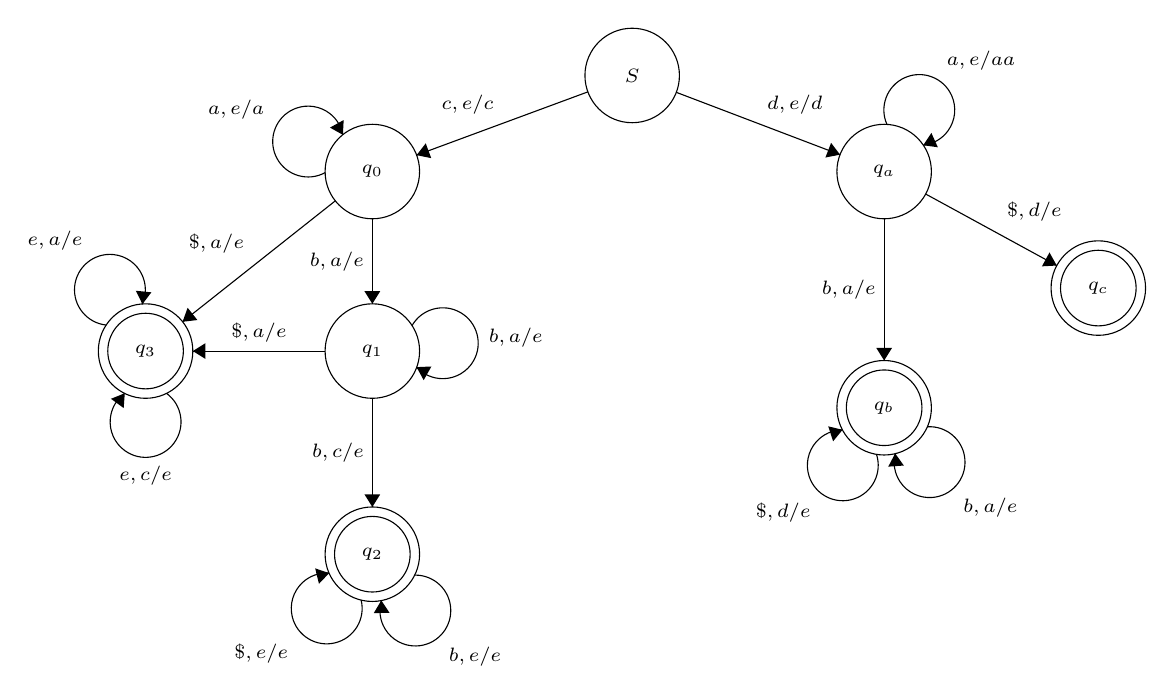
\begin{tikzpicture}[scale=0.2]
\tikzstyle{every node}+=[inner sep=0pt]
\draw [black] (39.9,-6.1) circle (3);
\draw (39.9,-6.1) node {$S$};
\draw [black] (23.4,-12.2) circle (3);
\draw (23.4,-12.2) node {$q_0$};
\draw [black] (55.9,-12.2) circle (3);
\draw (55.9,-12.2) node {$q_a$};
\draw [black] (23.4,-23.6) circle (3);
\draw (23.4,-23.6) node {$q_1$};
\draw [black] (23.4,-36.5) circle (3);
\draw (23.4,-36.5) node {$q_2$};
\draw [black] (23.4,-36.5) circle (2.4);
\draw [black] (9,-23.6) circle (3);
\draw (9,-23.6) node {$q_3$};
\draw [black] (9,-23.6) circle (2.4);
\draw [black] (55.9,-27.2) circle (3);
\draw (55.9,-27.2) node {$q_b$};
\draw [black] (55.9,-27.2) circle (2.4);
\draw [black] (69.5,-19.6) circle (3);
\draw (69.5,-19.6) node {$q_c$};
\draw [black] (69.5,-19.6) circle (2.4);
\draw [black] (37.09,-7.14) -- (26.21,-11.16);
\fill [black] (26.21,-11.16) -- (27.14,-11.35) -- (26.79,-10.41);
\draw (29.45,-8.59) node [above] {$c,e/c$};
\draw [black] (42.7,-7.17) -- (53.1,-11.13);
\fill [black] (53.1,-11.13) -- (52.53,-10.38) -- (52.17,-11.31);
\draw (50.23,-8.6) node [above] {$d,e/d$};
\draw [black] (20.412,-12.264) arc (298.96341:10.96341:2.25);
\draw (16.57,-8.3) node [left] {$a,e/a$};
\fill [black] (21.53,-9.87) -- (21.58,-8.93) -- (20.71,-9.41);
\draw [black] (23.4,-15.2) -- (23.4,-20.6);
\fill [black] (23.4,-20.6) -- (23.9,-19.8) -- (22.9,-19.8);
\draw (22.9,-17.9) node [left] {$b,a/e$};
\draw [black] (25.917,-21.99) arc (150.34019:-137.65981:2.25);
\draw (30.76,-22.75) node [right] {$b,a/e$};
\fill [black] (26.21,-24.62) -- (26.66,-25.45) -- (27.15,-24.58);
\draw [black] (23.4,-26.6) -- (23.4,-33.5);
\fill [black] (23.4,-33.5) -- (23.9,-32.7) -- (22.9,-32.7);
\draw (22.9,-30.05) node [left] {$b,c/e$};
\draw [black] (26.077,-37.828) arc (91.35757:-196.64243:2.25);
\draw (29.92,-42.36) node [below] {$b,e/e$};
\fill [black] (23.97,-39.43) -- (23.49,-40.24) -- (24.49,-40.22);
\draw [black] (22.686,-39.402) arc (13.89909:-274.10091:2.25);
\draw (16.35,-42.16) node [below] {$\$,e/e$};
\fill [black] (20.66,-37.7) -- (19.77,-37.4) -- (20.01,-38.38);
\draw [black] (20.4,-23.6) -- (12,-23.6);
\fill [black] (12,-23.6) -- (12.8,-24.1) -- (12.8,-23.1);
\draw (16.2,-23.1) node [above] {$\$,a/e$};
\draw [black] (21.05,-14.06) -- (11.35,-21.74);
\fill [black] (11.35,-21.74) -- (12.29,-21.63) -- (11.67,-20.85);
\draw (13.5,-17.4) node [above] {$\$,a/e$};
\draw [black] (10.323,-26.28) arc (54:-234:2.25);
\draw (9,-30.85) node [below] {$e,c/e$};
\fill [black] (7.68,-26.28) -- (6.8,-26.63) -- (7.61,-27.22);
\draw [black] (6.509,-21.949) arc (264.19932:-23.80068:2.25);
\draw (3.25,-17.26) node [above] {$e,a/e$};
\fill [black] (8.8,-20.62) -- (9.37,-19.87) -- (8.38,-19.77);
\draw [black] (55.9,-15.2) -- (55.9,-24.2);
\fill [black] (55.9,-24.2) -- (56.4,-23.4) -- (55.4,-23.4);
\draw (55.4,-19.7) node [left] {$b,a/e$};
\draw [black] (56.081,-9.217) arc (204.25512:-83.74488:2.25);
\draw (62.05,-5.84) node [above] {$a,e/aa$};
\fill [black] (58.38,-10.53) -- (59.31,-10.66) -- (58.9,-9.75);
\draw [black] (58.633,-28.409) arc (93.85757:-194.14243:2.25);
\draw (62.65,-32.87) node [below] {$b,a/e$};
\fill [black] (56.6,-30.1) -- (56.16,-30.94) -- (57.15,-30.87);
\draw [black] (55.41,-30.148) arc (18.29775:-269.70225:2.25);
\draw (49.49,-33.18) node [below] {$\$,d/e$};
\fill [black] (53.26,-28.6) -- (52.35,-28.38) -- (52.66,-29.33);
\draw [black] (58.54,-13.63) -- (66.86,-18.17);
\fill [black] (66.86,-18.17) -- (66.4,-17.34) -- (65.92,-18.22);
\draw (65.44,-15.39) node [above] {$\$,d/e$};
\end{tikzpicture}
\end{center}


Dpda of $L_2$:\\

\begin{center}
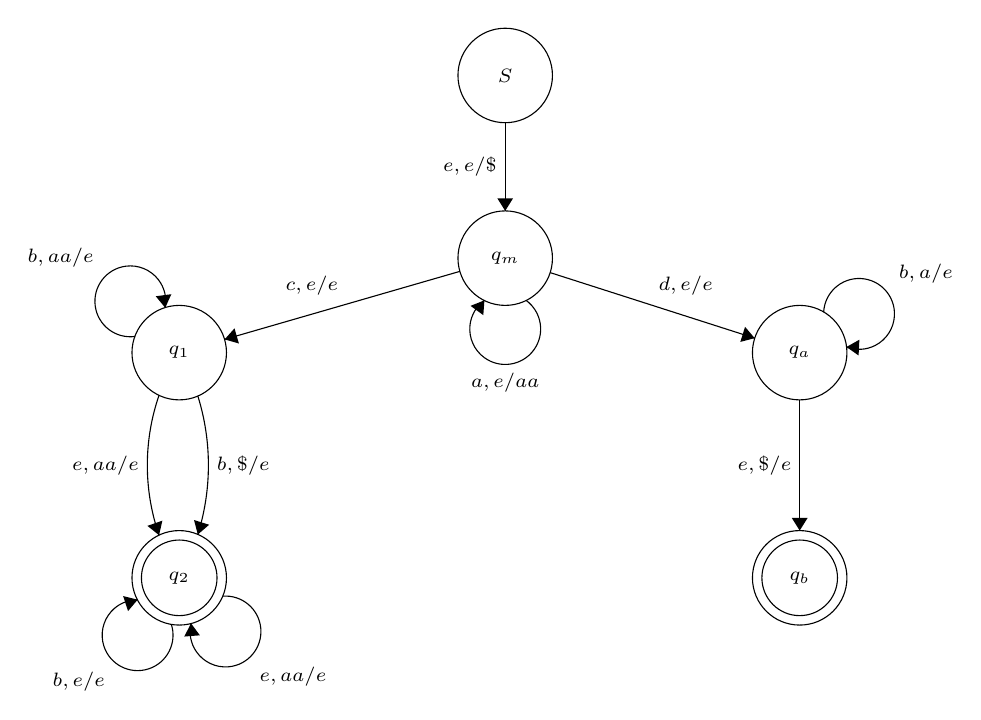
\begin{tikzpicture}[scale=0.2]
\tikzstyle{every node}+=[inner sep=0pt]
\draw [black] (39.9,-6.1) circle (3);
\draw (39.9,-6.1) node {$S$};
\draw [black] (39.9,-17.7) circle (3);
\draw (39.9,-17.7) node {$q_m$};
\draw [black] (19.2,-23.7) circle (3);
\draw (19.2,-23.7) node {$q_1$};
\draw [black] (58.6,-23.7) circle (3);
\draw (58.6,-23.7) node {$q_a$};
\draw [black] (19.2,-38) circle (3);
\draw (19.2,-38) node {$q_2$};
\draw [black] (19.2,-38) circle (2.4);
\draw [black] (58.6,-38) circle (3);
\draw (58.6,-38) node {$q_b$};
\draw [black] (58.6,-38) circle (2.4);
\draw [black] (39.9,-9.1) -- (39.9,-14.7);
\fill [black] (39.9,-14.7) -- (40.4,-13.9) -- (39.4,-13.9);
\draw (39.4,-11.9) node [left] {$e,e/\$$};
\draw [black] (41.223,-20.38) arc (54:-234:2.25);
\draw (39.9,-24.95) node [below] {$a,e/aa$};
\fill [black] (38.58,-20.38) -- (37.7,-20.73) -- (38.51,-21.32);
\draw [black] (37.02,-18.54) -- (22.08,-22.86);
\fill [black] (22.08,-22.86) -- (22.99,-23.12) -- (22.71,-22.16);
\draw (27.62,-20.07) node [above] {$c,e/e$};
\draw [black] (42.76,-18.62) -- (55.74,-22.78);
\fill [black] (55.74,-22.78) -- (55.13,-22.06) -- (54.83,-23.02);
\draw (51.36,-20.1) node [above] {$d,e/e$};
\draw [black] (16.394,-22.672) arc (277.60282:-10.39718:2.25);
\draw (11.67,-18.33) node [above] {$b,aa/e$};
\fill [black] (18.31,-20.85) -- (18.7,-19.99) -- (17.71,-20.12);
\draw [black] (60.122,-21.128) arc (177.11134:-110.88866:2.25);
\draw (64.87,-18.69) node [right] {$b,a/e$};
\fill [black] (61.57,-23.34) -- (62.34,-23.88) -- (62.39,-22.88);
\draw [black] (17.919,-35.294) arc (-160.96534:-199.03466:13.627);
\fill [black] (17.92,-35.29) -- (18.13,-34.37) -- (17.18,-34.7);
\draw (16.67,-30.85) node [left] {$e,aa/e$};
\draw [black] (20.381,-26.452) arc (17.38365:-17.38365:14.72);
\fill [black] (20.38,-35.25) -- (21.1,-34.63) -- (20.14,-34.33);
\draw (21.55,-30.85) node [right] {$b,\$/e$};
\draw [black] (21.951,-39.166) arc (94.76761:-193.23239:2.25);
\draw (26.42,-43.6) node [below] {$e,aa/e$};
\fill [black] (19.95,-40.89) -- (19.52,-41.73) -- (20.51,-41.65);
\draw [black] (18.696,-40.946) arc (18.02678:-269.97322:2.25);
\draw (12.82,-43.96) node [below] {$b,e/e$};
\fill [black] (16.56,-39.39) -- (15.64,-39.16) -- (15.95,-40.11);
\draw [black] (58.6,-26.7) -- (58.6,-35);
\fill [black] (58.6,-35) -- (59.1,-34.2) -- (58.1,-34.2);
\draw (58.1,-30.85) node [left] {$e,\$/e$};
\end{tikzpicture}
\end{center}

\subsection*{b.} 

Let's s represent the given languages with:\\

Regular = R\\
Context-free = C\\
The class of the complements of context-free languages = CC\\
Deterministic context-free = D\\


The things we must consider when constructing the Venn Diagram:\\
$-$ Every regular language is a context-free language. So regular languages are a proper subset of context-free languages.\\
\\
$-$ Every regular language is a deterministic context-free language. So regular languages are a proper subset of deterministic context-free languages.\\
\\
$-$ Every  deterministic context-free language is a deterministic context-free language. So deterministic context-free are a proper subset of context-free languages. An example for this proposition can be; L = (wwR), which is a context-free language but not deterministic, and L = (wcwR), which is both a deterministic context-free language and a context free language.\\
\\
$-$ In order to find the relation of complement with the other ones, we must look for closure rules of the other ones. Both regular and deterministic context-free languages are closed under complementation, so they are both proper subsets of the class of the complements of context-free languages. However,  context-free languages are not closed under complementation which means there are context-free languages that are not in the class of the complements of context-free languages.\\
\\
Thus, if we consider all of the propositions above, we will get a Venn Diagram which looks like:\\

\begin{center}
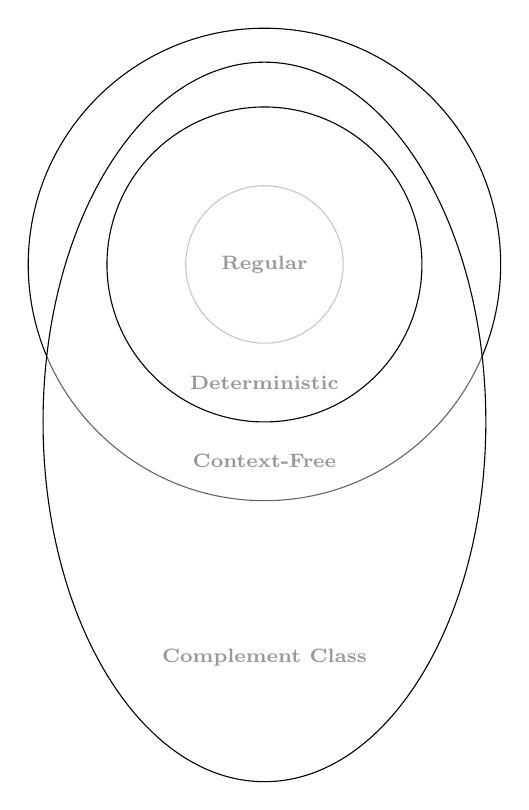
\begin{tikzpicture}
%% You can adjust the opacity here. For venn diagrams it is convenient to have a low opacity so that you can see intersections
	\begin{scope} [fill opacity = .4]
%% The draw command knows a lot of shapes. To make a rectangle you just need to specify two diagonal corners. Make sure you always have a semicolon at the end of your draw commands, otherwise latex flips out.
    %\draw (-5,5) rectangle (5,-6);
%% Similarly, you can make a circle by specifying the center and then the radius. You can also add a fill color, but if you're printing in black and white you'll probably want to remove that line.
    \draw[fill=white, draw = black] (0,0) circle (1);
    \draw[fill=white, draw = black] (0,0) circle (3);
    \draw[fill=white, draw = black] (0,-2) ellipse (80pt and 130pt);
    \draw[fill=white, draw = black] (0,0) circle (2);
%% We can use the node command to label points. If you put your cursor on "LARGE" or "textbf" a box will drop down with size and text style options.
   % \node at (-4,5.2) {\LARGE\textbf{X}};
    \node at (0,0) {\textbf{Regular}};
    \node at (0,-2.5) {\textbf{Context-Free}};
    \node at (0,-5) {\textbf{Complement Class}};
    \node at (0,-1.5) {\textbf{Deterministic}};
    \end{scope}
%% And now you have a venn diagram. Yay!
%\draw[help lines](-5,5) grid (5,-6);    This line can draw the grid lines to help guide you. I use these when I'm writing the code and then delete this line when I publish the pdf.
\end{tikzpicture}

\end{center}




\end{document}
